\documentclass[a4paper,12pt]{article}
\usepackage[utf8x]{inputenc}
\usepackage{amssymb}
\usepackage{amsfonts}
\usepackage{mathrsfs}
\usepackage{amsmath}
\usepackage{amsthm}
\usepackage[a4paper]{geometry}
\geometry{verbose,tmargin=0.5in,bmargin=0.5in,lmargin=0.51in,rmargin=0.51in,headheight=0.5cm,headsep=1.5cm,footskip=0.7cm}
\usepackage{times}
\usepackage{graphicx}
\usepackage{enumitem}
\usepackage{fancyhdr}
\usepackage{hyperref}
\usepackage{setspace}
\usepackage{subcaption}
\usepackage{mathtools}
\usepackage[square,sort,comma,numbers]{natbib}
\setlength{\bibsep}{0.0pt}

%\pagestyle{fancy}
%\fancyhf{}
%\lhead{Thomas Delaney}
%\rhead{COSYNE 2018 Abstract}
%\cfoot{\thepage}

\newtheorem{theorem}{Theorem}
\newtheorem{proposition}{Proposition}[section]
\newtheorem{lemma}{Lemma}[section]
\newtheorem{corollary}{Corollary}[section]
\theoremstyle{definition}
\newtheorem{definition}{Definition}[section]

\newcommand{\boldnabla}{\mbox{\boldmath$\nabla$}} % to be used in mathmode
\newcommand{\cbar}{\overline{\mathbb{C}}}% to be used in mathmode
\newcommand{\diff}[2]{\frac{d #1}{d #2}}% to be used in mathmode
\newcommand{\difff}[2]{\frac{d^2 #1}{d #2^2}}% to be used in mathmode
\newcommand{\pdiff}[2]{\frac{\partial #1}{\partial #2}} % to be used in mathmode
\newcommand{\pdifff}[2]{\frac{\partial^2 #1}{\partial #2^2}}% to be used in mathmode
\newcommand{\upperth}{$^{\mbox{\footnotesize{th}}}$}%to be used in text mode
\newcommand{\vect}[1]{\mathbf{#1}}% to be used in mathmode
\newcommand{\curl}[1]{\boldnabla \times \vect{#1}} % to be used in mathmode
\newcommand{\divr}[1]{\boldnabla \cdot \vect{#1}} %to be used in mathmode
\newcommand{\modu}[1]{\left| #1 \right|} %to be used in mathmode
\newcommand{\brak}[1]{\left( #1 \right)} % to be used in mathmode
\newcommand{\comm}[2]{\left[ #1 , #2 \right]} %to be used in mathmode
\newcommand{\dop}{\vect{d}} %to be used in mathmode
\newcommand{\cov}{\text{cov}} %to be used in mathmode
\newcommand{\var}{\text{var}} %to be used in mathmode
\newcommand{\mb}{\mathbf} %to be used in mathmode
\newcommand{\bs}{\boldsymbol} %to be used in mathmode
% Title Page
\title{How informative are retinal ganglion cells?}
\author{Thomas Delaney 1330432}

\begin{document}

\noindent
\textbf{Title:} Does structure in neural correlations match anatomical structure during spontaneous behaviour?
\vspace{-0.5cm}
\subsubsection*{300-word Summary}
\vspace{-0.3cm}
Information in the brain is carried in correlated network activity\cite{cohen1, cohen2}. Recent findings show that spontaneous behaviours explain correlations in parts of the brain not usually related to motor control\cite{stringer}. The question arises, are correlated networks restricted to anatomical brain regions? We found that correlated networks tend to exist \textit{within} anatomical regions at short time-scales, and \textit{across} anatomical regions at longer time-scales. This implies that neural circuits compute locally at short time-scales ($\sim 50$ms) but more globally at longer ($\sim 1$s) time-scales. 

Because of limitations in recording technology most research has explored correlations between neurons within a given brain region. Relatively little is known about correlations between neurons in different brain regions. However, the recent development of `Neuropixels' probes\cite{jun} has allowed extracellular voltage measurements to be collected from multiple brain regions simultaneously routinely, and in larger numbers than traditional methods. We used a publicly available Neuropixels dataset to analyse correlations between different brain regions.

Using eight probes each in three mice, readings from 2296, 2668, and 1462 cells respectively in nine brain regions were extracted during 1 hour of activity. Each mouse was behaving spontaneously and could use their front paws to turn a wheel\cite{stringer}. We examined pairwise spike count correlations between neurons within the same region, and between neurons in different regions. We found that cells from the same region tend to be more strongly correlated than cells from different regions. This difference in correlation strength is greater for shorter time-scales, and weakens at longer time-scales. 

We used a cutting-edge method\cite{humphries} to detect communities in the network induced by pairwise correlations. In agreement with our first finding, at shorter time-scales we found many communities dominated by cells from a single region. At longer time-scales, communities spanned multiple brain regions. 

\vspace{-0.5cm}
\subsubsection*{Additional Detail}
\vspace{-0.3cm}
The three mice from which the data were collected had some key differences. The first mouse was a female wild type, P73. The second mouse was a male mutant (TetO-GCaMP6s, Camk2a-tTa), P113. The third mouse was a male mutant (Ai32, Pvalb-Cre), P99.

Prior to measuring spike count correlations, we chose suitable time bin widths for binning the spike counts by taking a similar approach to \cite{cohen2}. We evaluated the average correlations from many cell pairs using different values for the time bin width. We found that correlations increased logarithmically with the size of the bin width consistently across mice. We used a bin width of $2$s in order to capture the magnitude of the correlations, without completely averaging out short-term dynamics. However, we still performed our analyses at time bin widths ranging from $50$ms to $3$s in order to assess the effect of the bin width. The same dataset was used in \cite{stringer}; they used $1.2$s time bins for their analyses.

% revisit
To assess the correlation significance, we measured the shuffled correlation between each pair. We found that the mean correlation was usually an order of magnitude greater than the mean shuffled correlation. 

% disposable
Due to the large number of cells, and the even larger number of cell pairs, in order to make these measurements in a reasonable amount of time, a local supercomputer was used to perform the calculations using parallelisation to speed up the process.

To compare \textit{within-region} mean correlations to \textit{between-region} mean correlations, we created correlation matrices with within-region correlations on the main diagonal and between-region correlations elsewhere. There appeared to be no consistency in correlation patterns across mice. % (see figure \ref{fig:regional_correlation_matrices}).

%\begin{figure}[t!]
%    \centering
%    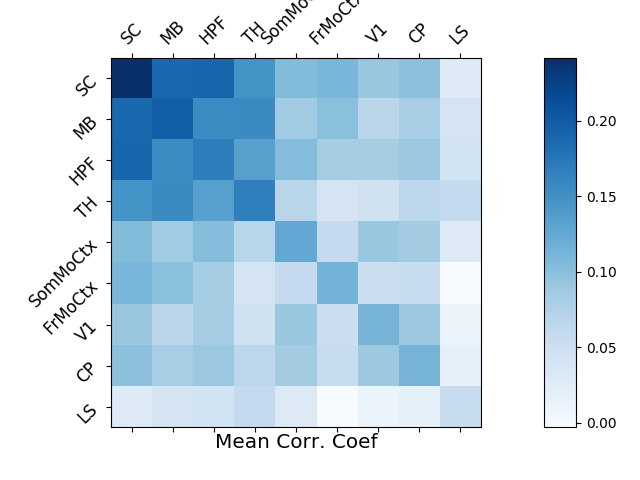
\includegraphics[width=0.32\columnwidth]{images/Krebs_2p0_corr.png}
%    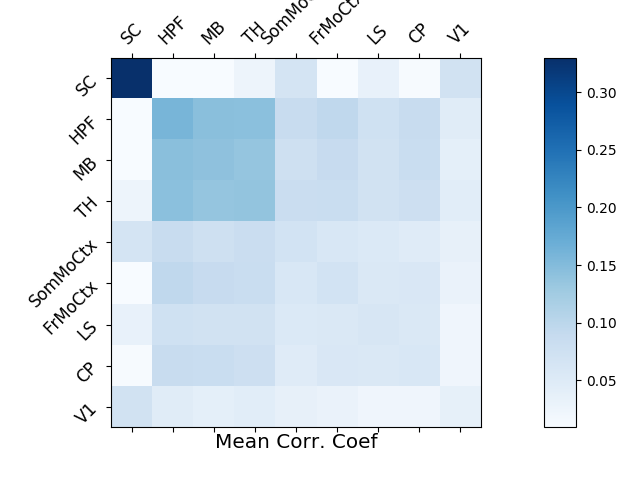
\includegraphics[width=0.32\columnwidth]{images/Robbins_2p0_corr.png}
%    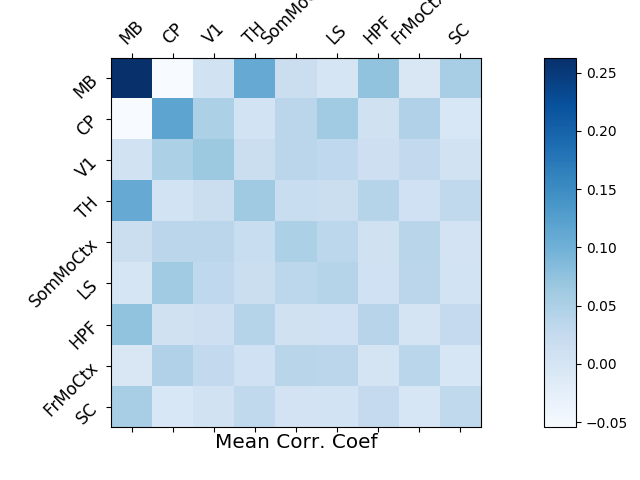
\includegraphics[width=0.32\columnwidth]{images/Waksman_2p0_corr.png}
%    \caption{Matrices showing the mean spike count correlation taken across pairs of neurons from various brain regions. One matrix for each mouse. Entries on the main diagonal correspond to pairs where each cell is from the same region. All other entries have pairs of cells from different regions.}
%    \label{fig:regional_correlation_matrices}
%\end{figure}

We compared within-region correlations to between-region correlations at different time-scales by using different values for the time bin width. For a given region, we found that within-region mean correlations tended to exceed most or all of the mean correlations for between-region correlations involving that region. We also found that this tendency was greatest for shorter time bins, and reduced for longer time bins (fig. \ref{fig:within_between}). This dynamic may reflect the dispersion of correlations throughout the brain over time.

\begin{figure}[t!]
    \centering
    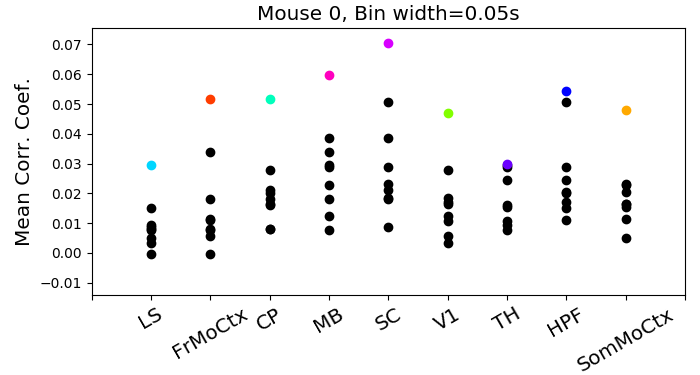
\includegraphics[width=0.45\columnwidth]{images/Krebs_0p05_corr_comp.png}
    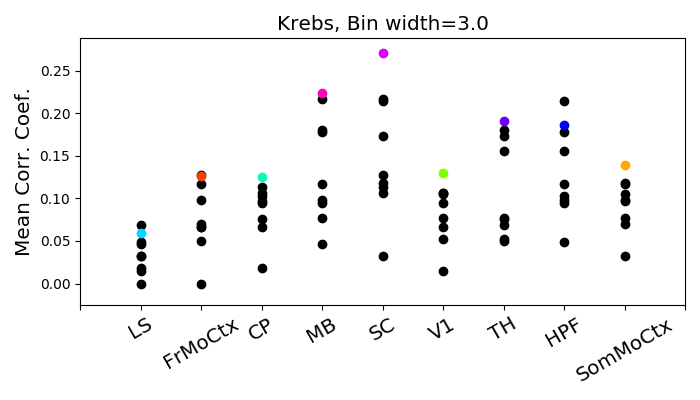
\includegraphics[width=0.45\columnwidth]{images/Krebs_3p0_corr_comp.png}
    \vspace{-0.4cm}
    \caption{Regional comparisons of within-region (coloured dots) and between-region (black dots) correlations for the same mouse using different time bin widths. Each black dot represents the mean correlation for a mixed region pair. For example, one of the black dots above `LS' represents the mean correlation of cell pairs where one cell is from the LS, and the other is from V1. There is a corresponding black dot above V1 for the same value. The reduction in difference between within-region and between-region mean correlations with increasing time bin width shown here was also observed at intermediate values for the time bin width ($0.2$s, $1$s, $2$s, $3$s).}
    \vspace{-0.4cm}
    \label{fig:within_between}
\end{figure}


The cutting-edge community detection method that we used involved choosing a null network distribution and testing if this model was valid for the data network. Choosing a null model allowed us to conserve network strength, degree sequence, and sparsity of the data network in our null model. The hypothesis testing allowed us to determine if the data network contained structure beyond that described by the null model. It also allowed us to determine a subspace to the data network vector space where this structure exists, and which nodes contribute to this structure. Thus we could remove those nodes not contributing to the extra structure, and perform the community detection algorithm in the subspace. This process is referred to as \textit{Network Noise Rejection} \cite{humphries}. The community detection itself is analogous to ensemble methods for time-series analysis. It uses the output of many different modularity clustering attempts to find one final clustering through \textit{consensus-clustering}.

We performed the network noise rejection and community detection on weighted networks created by spike count correlation measurements. We did this using different values for the time bin width. We found that correlated communities generally included neurons from multiple brain regions. But, we found that communities dominated by neurons from a single region were more likely to be observed when using a smaller time bin width (fig. \ref{fig:regional_cluster_maps}). This result may also reflect dispersion of correlations throughout the brain over time.

\begin{figure}[t!]
    \centering
    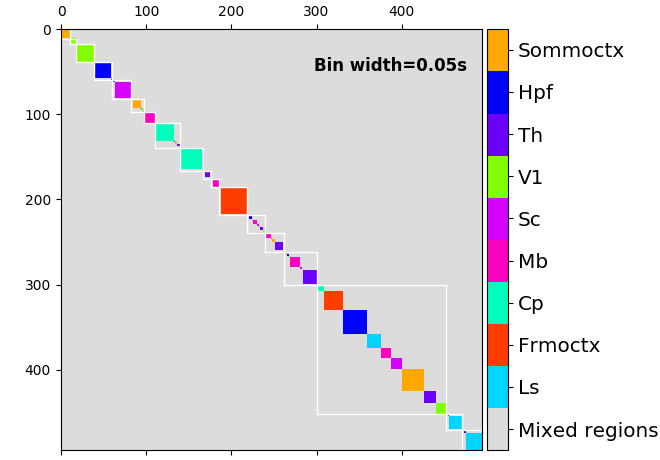
\includegraphics[width=0.45\columnwidth]{images/Krebs_0p05_regional_cluster_map.png}
    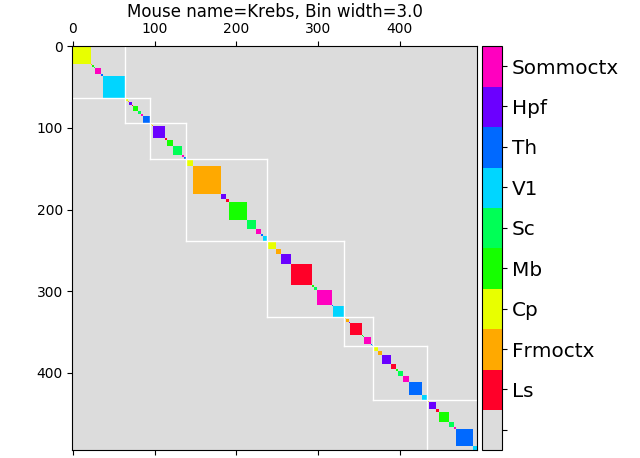
\includegraphics[width=0.45\columnwidth]{images/Krebs_3p0_regional_cluster_map.png}
    \vspace{-0.3cm}
    \caption{Matrices showing cell regional membership and community membership for the same mouse using different bin widths. Each cell has a corresponding row and column. Regional membership is denoted by colour. The majority of cell pairs are between regions and are therefore grey. Network communities are those cells within the white borders. Each cell is in one community only. In general, communities include pairs from multiple regions. But, at shorter time-scales (left-panel) communities dominated by a single region are more prevalent.}
    \vspace{-0.6cm}
    \label{fig:regional_cluster_maps}
\end{figure}


\vspace{-0.6cm}
\renewcommand\refname{\normalsize References \vspace{-0.5cm}}
\bibliography{cosyne_2020_application.bbl}
\bibliographystyle{rsc}

%  \item correlation histogram results largely agree with previous findings, cite cohen and kohn.
\end{document}
